\documentclass{ximera}
\input{../../preamble.tex}
\license{Creative Commons 3.0 By-NC}
\outcome{ Define a critical point.}
\outcome{ Find critical points.}
\outcome{ Define absolute maximum and absolute minimum.}
\outcome{ Find the absolute max or min of a continuous function on a closed interval.}
\outcome{ Define local maximum and local minimum.}
\outcome{ Compare and contrast local and absolute maxima and minima.}
\outcome{ Identify situations in which an absolute maximum or minimum is guaranteed.}
\outcome{ Classify critical points.}
\outcome{ State the First Derivative Test.}
\outcome{ Apply the First Derivative Test.}
\begin{document}

\begin{exercise}

	The graph of $y=f'(x)$ is below, for a function $f$.
	\begin{center}
		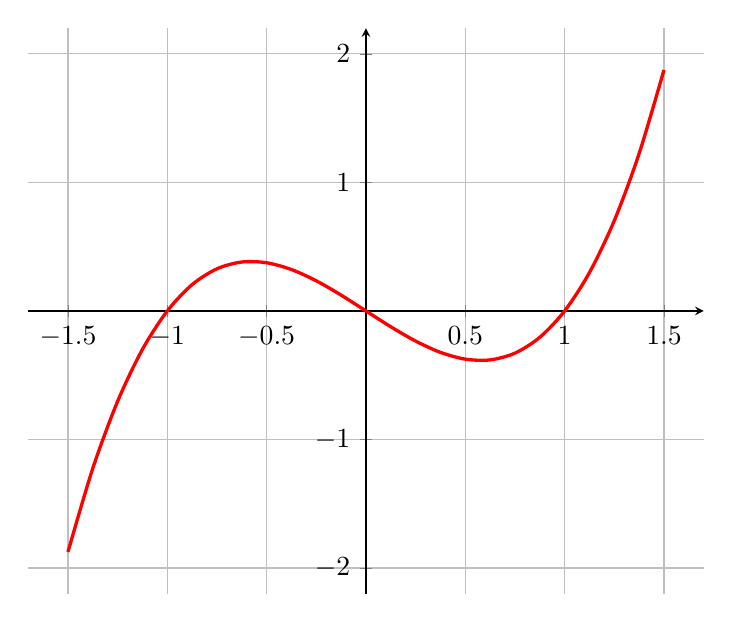
\begin{tikzpicture}[scale=1]
			\begin{axis}[
				xmin=-1.7, xmax=1.7, ymin=-2.2,ymax=2.2,    
				axis lines =middle, 
				every axis y label/.style={at=(current axis.above origin),anchor=south},
				every axis x label/.style={at=(current axis.right of origin),anchor=west},
				xtick={-1.5,-1,...,1.5}, ytick={-2,..., 2},
				grid=major, width=4in,
				]
				\addplot[color=red, very thick, smooth, domain=-1.5:1.5]{x^3-x};
			\end{axis}
		\end{tikzpicture}
	\end{center}	

	How many critical points does $f$ have? $\answer{3}$.
	\begin{exercise}
		List them, from smallest to largest.
		\[ \answer{-1} \,\, , \,\, \answer{0} \,\, , \,\, \answer{1} \]

		\begin{exercise}
			Classify the critical points.

			$x=-1$ is \wordChoice{\choice[correct]{a local minimum}\choice{a local maximum}\choice{not a local extremum}}.
			
			$x=0$ is \wordChoice{\choice{a local minimum}\choice[correct]{a local maximum}\choice{not a local extremum}}.
			
			$x=1$ is \wordChoice{\choice[correct]{a local minimum}\choice{a local maximum}\choice{not a local extremum}}.			
		\end{exercise}
	\end{exercise}
	
\end{exercise}
\end{document}
